\label{sec:data}
% Main characteristics of the data set: source, type of data
% Description of variables used for the	analysis and correspondence with the (ideal) magnitudes in the empirical specification
% Descriptive statistics of the	main variables in the analysis
The data used in the analysis is comprised of data from multiple sources. We utilize three 'types' of data:
\begin{itemize}
    \item Data on airports. In the network setting, these correspond to nodes in the network. 
    \item Data on flights. These dataset contain information on flights between airports. As will be described in detail below, we have access to a rich dataset on US flights. In the network setting, this information corresponds to links in the network.
    \item Prices. Data on prices is generally harder to obtain. For this reason, we have chosen to scrape web-data on prices from \textit{Skyscanner}.
\end{itemize}

\subsection{Airport Data}
Data on airports comes from OpenFlights.\footnote{Available at: \url{https://openflights.org/data.html}} The dataset contains airport IATA code, name, city, country, geographical location (crs: WTS84), as well as a unique OpenFlights identifier, ICAO code and altitude. The dataset contains information on a total of 7698 airports worldwide, of which 1518 are located in the United States. Throughout the analysis, we focus on the airports that are found at least once in our dataset on flights, which is a total of 358 airports in 2018.
%Data on airports comes from two overlapping sources. Firstly, we have a dataset from the 2009 Statistical Computing Data Expo\footnote{Available at \url{http://stat-computing.org/dataexpo/2009/}}. This dataset contains information 3376 US airports, and the unique IATA\footnote{International Air Transport Association} code, airport name, city, country and geographical location in WTS84 coordinates. This dataset contains 3.376 observations of individual airports. As will be described in \ref{subsec:Flight_Data}, we only have information on flights/connections to and from a subset of these. A likely explanation is, that a number of these airports are not used for commercial air transport, but rather for e.g. training/sports purposes.\par
% Tjek at det reelt er WTS84 koordinater - det ser sådan ud.
%Secondly, we have a dataset on airports from OpenFlights\footnote{Available at: \url{https://openflights.org/data.html}}. This dataset contains the same information as the above, but further includes inter alia a unique 'OpenFlights identifier', ICAO code, and altitude. Furthermore, this dataset contains airports from all over the world.

%We will primarily use the OpenFlights data, whenever the analysis has a global scope. This dataset contains information on 7543 individual airports.

\subsection{Flights Data}
\label{subsec:Flight_Data}
Flight data comes from the Bureau of Transportation Statistics (\citet{BTS}). The dataset covers all scheduled fligths by carriers (airlines) that account for at least one percent of domestic scheduled passenger revenues. We have flight data for 1998, 2007 and 2018. Each of the datasets include information on several million commercial flights within the US. For each flight, we have a range of information, including the aircraft carrier, origin and destination (IATA coded), distance travelled, time in air date etc. Flight data can be merged with airport data using the IATA codes on airports. \medskip\\
We only use the 1998 and 2007 data to assess how the network has changed over time.

%% Update: Flights data fra bts.gov og fra stat-comp (men det er igen fra bts.gov).
% Airports data: Bruger kun OpenFlights datasættet. 


%Data on airports and connections is available at: \href{https://openflights.org/data.html}{openflights.org/data.html}. See Figure \ref{fig:airports} below. The dataset includes an airport identifier (IATA code), location data (latitude and longitude), and various characteristics of the airport (country, city, altitude etc.).
%Furthermore, the dataset contains connections between airports (67,663 routes between 3,321 airports on 548 airlines). %Airports are identified using the IATA code.%we already mentioned this above
%\medskip\\
%Data on prices are scraped from the internet. Various sites contain flight prices (Skyscanner, Momondo, Flightfinder, Expedia mv.). Our choice of site will be guided by practical concerns.
%\par
%Alternative data:  \url{http://stat-computing.org/dataexpo/2009/}
%\begin{figure}[H]
%  \centering
%  \caption{Airports}
%    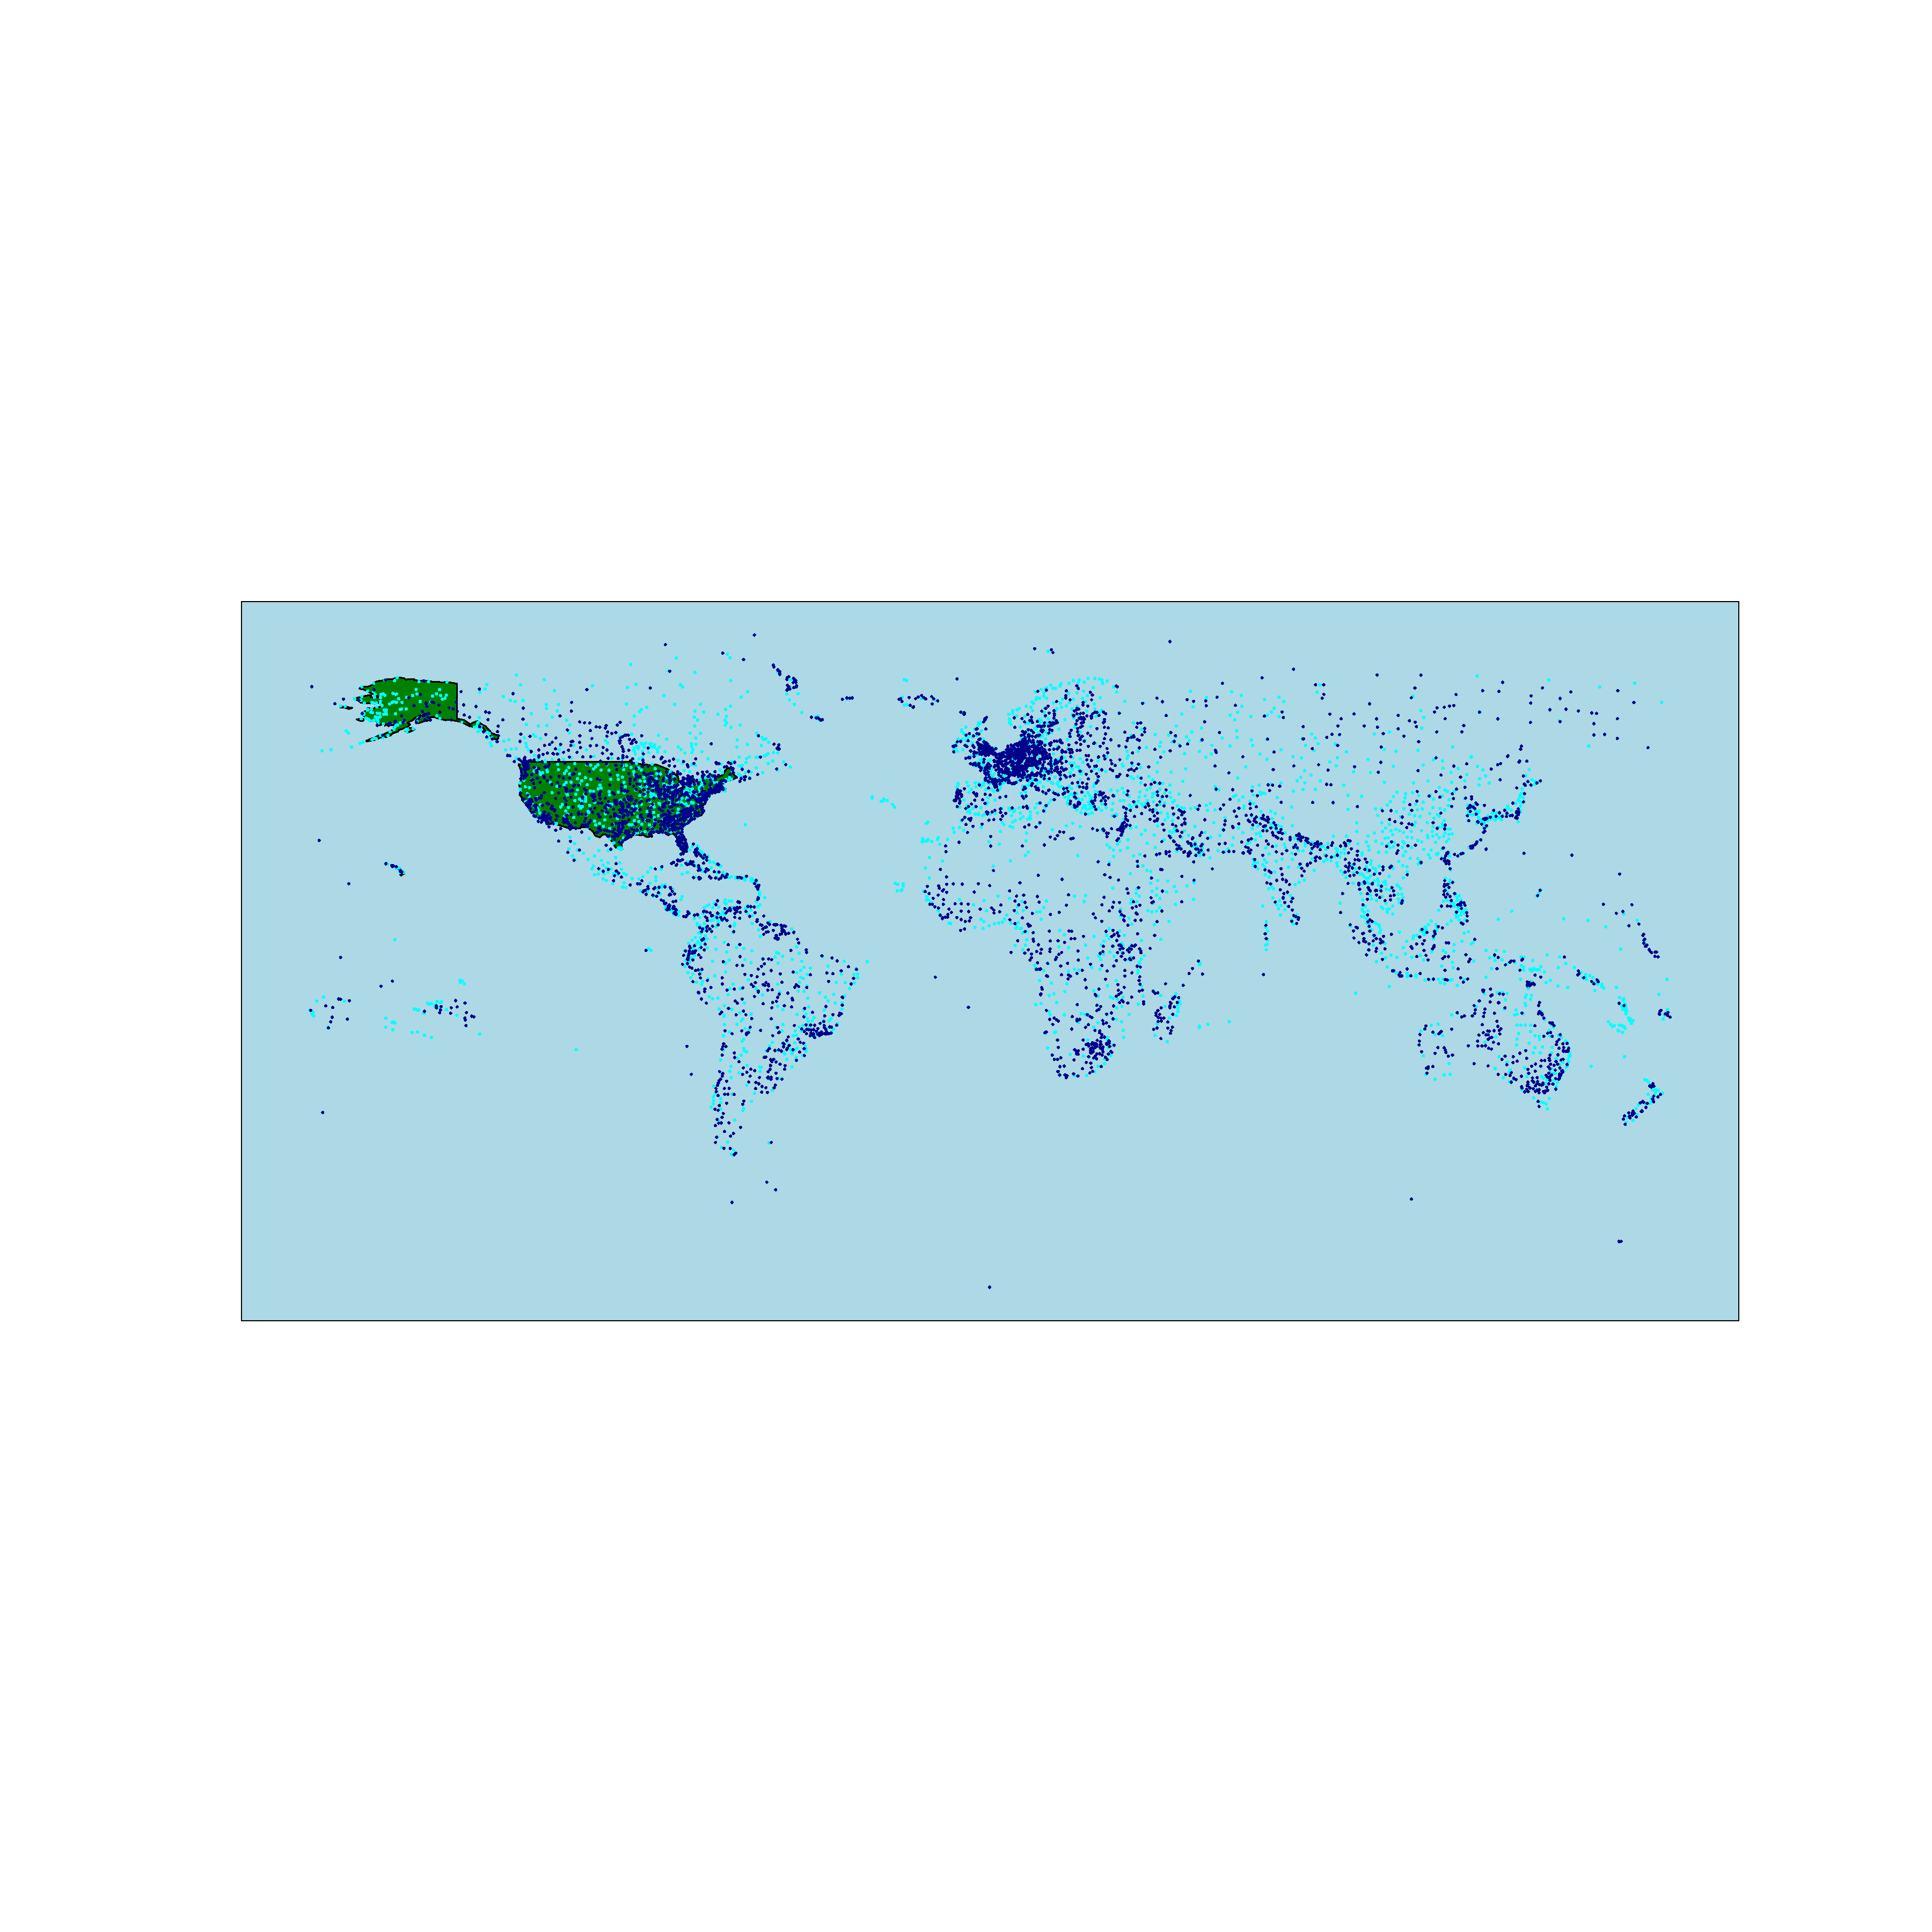
\includegraphics[width=1. \textwidth]{Exam/Airports_WorldMap}
%  \label{fig:airports}
%\end{figure}

\subsection{Price Data}
We scrape the price data from \url{skyscanner.com} using the \texttt{Selenium} package in Python. The scraper function launches a browser and opens the URL for a given flight at our chosen date which is May 27th. If possible the price of the cheapest direct flight is chosen. The prices of flights operated by Southwest Airlines are not shown at Skyscanner. If their flight is the only one operating, the price of the cheapest indirect flight is chosen. The cheapest indirect flight is also chosen if no carrier is operating a direct flight at the date. For routes where we could not find a price this date, the script is rerun for the next day, the 28th. In order to reduce the number of searches without result and thereby reduce time, we only choose routes with an average of more than one flight per week.\footnote{See github for documentation, \url{https://github.com/Morten-Esketveit/TSDS-gruppe-2019/tree/master/Exam}.}

There is a number of limitations to our approach. First, in order to reduce the scraping time, we are scraping prices for only 1 day. This implies that routes not operated on this particular Monday (and Tuesday) are not in the data set. Furthermore choosing one specific date is problematic since prices shows systematic changes across weekdays, and seasonality across the year. This approach is likely not to give an accurate measure of prices in general may cause our prediction model to perform badly. 

The price dataset consist of prices for 5.283 of the total 6.425 routes. There is a number routes that turn out to have extremely high prices. This is because these routes are operated by some sort of air taxi company. Modelling these prices is beyond the scope of this paper and therefore we remove them from the dataset. The final dataset consists of 5.083 observations.




